\chapter{Infrastructure} 
\label{chap:infrastructure}

\section{Distributed Systems Architecture}

When developing a digital infrastructure system, it is common to start with a
monolith approach where all application concerns are contained in a single
deployment, but it is hard to ignore its disadvantages as it can easily become
the bottleneck of the system. With monoliths, a lot more care has to be given to
how each part of the system communicates with one another, as communication is
achieved through method or function calls. This leads to very tight coupling
between different application components, which inevitably provides a lot of
friction to updating the codebase due to the high risk of it disabling the
service entirely.

Like with most applications, with every new feature the monolith grows, also
increasing the computing resources required to run a single instance. In times
of traffic peak, it is common for an application to scale its service allowing
for response speed to remain within acceptable times. The bigger the deployment,
the longer it takes to make a new instance available and the more computing
resources are used, making it more expensive to provide availability in times of
high traffic.

With this type of system, technological choices have a big impact on the final
product, and have to be thoroughly planned in the beginning to guarantee that
the system fulfills its requirements. It also makes it harder to adopt a
different technology further into the development due to the technological cost.
This point alone, makes it hard to accept this design, especially considering
the frequency of new advances in the field, and it is only natural that a new
approach to system architecture were developed.

Although there is no formal definition for what a microservice is,
\cite[Chapter~1]{newman2015building} states that ``Microservices are small,
autonomous services that work together.'' Small is of course a subjective
measure, but in fact there is no "theoretical" boundary on this quantity. It
depends on the context of the application and the business, but considering the
size of these microservices, it is only logical that each of the small services
follows some kind of team structure allowing for parallel development, without
any real coupling between the services. 

Microservices are built around different ``business capabilities'' which are
``independently deployable by fully automated deployment machinery''
\cite{MartinFowlerMicroservices}. In other words, each microservice can be
deployed on its own, hence scaling services and reliability is "included" with
this kind of architecture. This makes updating code very low risk. As an
example, in the scenario there is some flaw in a new deployment sent to
production, it will only affect that microservice in particular, making it
easier not only to track where the fault lies, but also guaranteeing that the
remaining services are not made fully unavailable.

When scaling smaller decoupled services, only the service that requires scaling
is in fact replicated. This leads to less computer resources utilization thanks
to the reduced overhead of the service, resulting in a considerate cost
reduction, and faster response to scaling needs.

With the possibility of running decoupled services interacting through
lightweight network calls, each microservice can be programmed in whichever
programming language and run the datastore that fits its needs best. The reduced
size of each service, also makes technological changes and code refactoring a
lot simpler, and can be done in a lot less time when compared to its counterpart.

It is also worth mentioning that the separation between each service allows
several representations of the same data in different ways depending on the
service that is storing it. The benefits of this approach are not only in a
projection perspective (there isn't a need to over-engineer how the data
will be stored for future purposes that still are not implemented), but it also
helps model the world in the way that fits each service best. 

Having multiple representations for the same data, also leads to inconsistency
in the data stored in different services. Employing a data warehouse in this
scenario overcomes this hurdle by unifying the data models of the different
services, and becoming the single source of truth for any representation of the
data within the system. It is also notably hard to maintain data consistency
between the distributed services, and on this note, the following section is
introduced.

\section{Distributed Messaging Systems}\label{sec:DMS}

When interacting between two distinct distributed servers, rarely should two
components communicate with one another directly or through synchronous
communication. If this were not the case, the communication would become too
convoluted with the increase of instances and services, becoming a source of
coupling, i.e., communication routes would have to be defined at the machine
level. 

As stated in \cite{sharvari2019study}, it is clear the market needs point to a
messaging system that has the following features:
\begin{itemize}
    \item Scalable - the system provides tools with which services can process a
        bigger load of messages in a time of intense volume of traffic;
    \item Space decoupling – The receiving and sending entity do not need to
        “know” each other;
    \item Reliable – The system can guarantee that the receiver has received the
        message;
    \item Asynchronous  – The sender and receiver do not have to be active at
        the same time.
\end{itemize}

To enable decoupling between services, most messaging systems leverage the use
of a broker, providing with the space and time decoupling, with the added
benefit of it also being asynchronous. After the broker acknowledges the
reception of the message sent by a producer, the producer does not need to
worry about its consumption allowing for it to go back to the tasks it has at
hand. There are two main approaches at solving this problem, event- and
message-driven paradigms.

\subsection{Message-Driven}

This paradigm makes use of message queues where producers send the data for it
to be consumed by a single consumer in the same order it was appended to the
queue. When data is produced, in case there isn’t a consumer interacting with
the queue, the message is stored until read. 

RabbitMQ is a well known platform commonly used for this purpose. All the
previous features are provided, and on the note of scalability, a given service
can connect to a queue with one or more consumers to increase consumption rate.
This is done using round-robin dispatching \cite{RabbitMQscale} which simplifies
parallelizing work between instances, always guaranteeing that each message in a
queue will be read by a single consumer.

\subsection{Event-Driven (Publish/Subscribe)}

Messaging system which allow a producer to send a message to a certain category,
which can be posteriorly retrieved by multiple consumers which are subscribed to
the same category. This architecture not only decouples the services, it also
allows many-to-many communication.

A common application for the event driven paradigm is for event sourcing. This
is the pattern of storing any event that changes a system's state via an event
object, onto an event log that preserves the sequence in which the events
occurred. This is presented as an alternative to storing structures that model
the state of the world, into storing events that lead to the current state of
the world \cite[Chapter~5]{nadareishvili2016microservice}.

Comparing this scenario to the one of using a database, in the latter, every
time the main database is updated, a second database recording the historic
state has to be updated as well, storing the past states the system has been
through. With event sourcing, when an event changes the state of the system, it
is simply appended to the sequential event log, which in turn makes it less
expensive to make operations of this type.

\section{Kafka}

Kafka functions as a distributed log running in multiple brokers that coordinate
with each other to form a cluster.

\begin{figure}[H] 
    \centering
    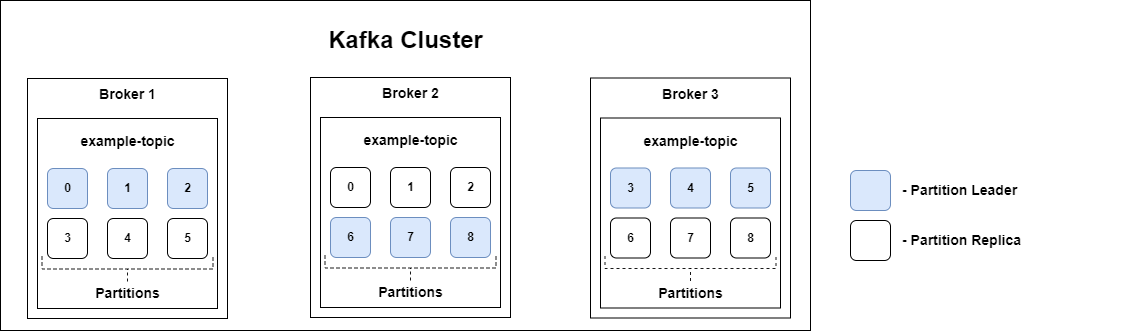
\includegraphics[width=\textwidth]{images/infrastructure/Kafka Cluster.png}
    \caption{
        Representation of a Kafka Cluster composed of three brokers, with a
        single topic (Example Topic), containing 9 partitions and a
        replication factor of 2.
    } 
    \label{fig:kafka_cluster} 
\end{figure}

\subsection{Broker}

A Kafka cluster is made up of one or more brokers, which function as servers
where the messages can be published to, and consumed from. This is the entity
each client has to connect to in order to interact with Kafka. After a client
connects to a single broker, it will also be connected to the remaining elements
of the cluster.

\subsubsection{Topics and Partitions}

When data is published, the producer has to specify to which topic the record
goes to. A topic contains several partitions, and each partition can be stored
in different brokers. Message order is only guaranteed within a single
partition.

At the time of topic creation, there are three parameters that have to be
provided: 
\begin{enumerate}
    \item \textbf{topic} - The name of the topic to create;
    \item \textbf{partitions} - The amount of partitions the topic is subdivided
        in;
    \item \textbf{replication-factor} - The amount of replicas of each partition.
\end{enumerate}
The \lstinline{example-topic} presented in figure \ref{fig:kafka_cluster} would have been
configured with \lstinline{topic=example-topic}, \lstinline{partitions=9} and
\lstinline{replication-factor=2}.

Although the first two parameters are self-explanatory, the third is one of the
most important features to guarantee a reliable service to a producer. 

Assuming the scenario of choosing the replication factor of 2, this means that
for each partition in the created topic, there will be 2 partitions that
represent the same log in different brokers. At any given time, there is only 1
partition leader (broker), which leaves the other partition trying to keep up
with the main log. When a replica is up-to-date with the leader, it becomes an
in-sync replica (ISR). If a partition leader fails unexpectedly, the partitions it is
leading have to be reassigned a different leader. For each partition, the new
partition leader will be one of the brokers that contains an in-sync replica of
the same partition.

\subsection{Producer}

To publish data, producers have to connect to one of the brokers from the
cluster, which will automatically inform the client as to how to connect to the
remaining brokers of the same cluster. When sending a record, the producer
has to specify the topic to which the record is to be added, and may optionally
provide other parameters which will impact the partition the record will be
added to. If no additional parameter is provided, a random partition is selected
to which the record is added.

\begin{figure}[hbt!] 
    \centering
    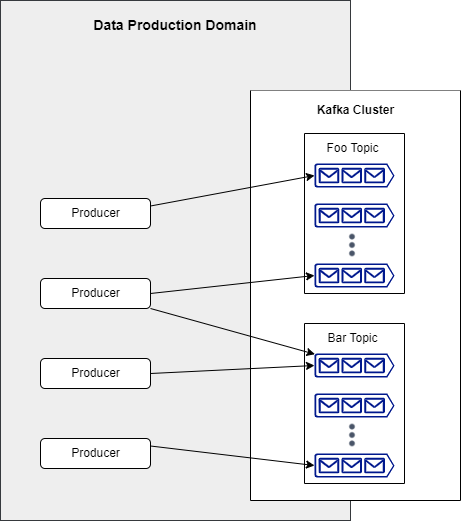
\includegraphics[width=0.5\textwidth]{images/infrastructure/Production Domain.png}
    \caption{
        Data production representation within the Kafka Ecosystem.
    } 
    \label{fig:data_production_domain} 
\end{figure}

For a single partition, the log that belongs to the partition leader (shaded
partitions in figure \ref{fig:kafka_cluster}) is where the messages are appended
to and read from. To guarantee a message is delivered safely to the cluster, a
producer might want to wait for acknowledgement. This is one of the
configurations that allows for reliability when adding a message to a topic
\cite{KafkaProducer}. In figure \ref{fig:data_production_domain}, the partitions
presented are only the leader partitions within the topic.

There are 3 possible values for this configuration:
\begin{itemize}
    \item \lstinline{acks=0} - Producer does not wait for acknowledgement, making it an
        unreliable configuration;
    \item \lstinline{acks=1} - Producer waits for acknowledgement from the partition
        leader;
    \item \lstinline{acks=all} - Producer expects an acknowledgement from leader and all
        of its replicas.
\end{itemize}

After appending data to a log, it can no longer be changed (immutability).
Additionally, when producing a message, if the order of a group of messages is
important, Kafka provides a feature that allows messages to be consumed in the
same order as they were produced. This is done by setting the key of a record to
the same value, having a hash function run over the key, and the partition where
the message goes to is consistently the same, while the number of partitions in
the topic does not change. If the number of partitions changes, this is no
longer the case.

\subsection{Consumer Group and Consumer Clients}
\label{sec:kafka_consumer_group}

When connecting a consuming client to the messaging system, the topic(s) it
wishes to subscribe to, the consumer group id and at least one of the brokers from
the cluster have to be provided (a connection to a single broker connects the
consumer to all the other brokers in the cluster). 

\begin{figure}[hbt!] 
    \centering
    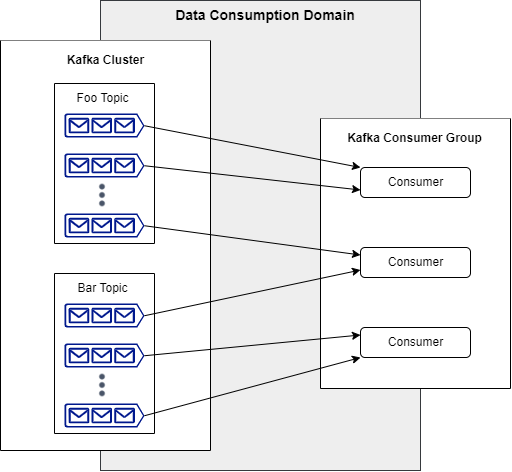
\includegraphics[width=0.6\textwidth]{images/infrastructure/Consumption Domain.png}
    \caption{
        Representation of the consumption process for a Kafka Consumer Group.
    } 
    \label{fig:data_consumption_domain} 
\end{figure}

Messages are then read in order w.r.t a single partition, and in parallel w.r.t.
multiple partitions. Each consumer from within a consumer group, reads from
exclusive partitions.  This means that two consumers belonging to the same
consumer group cannot be responsible for reading messages from the same
partition, which in turn implies that the parallelism Kafka provides, is through
the partitions in a topic. The amount of active consumers a single consumer
group can have is therefore limited to the total amount of partitions in the
topics the consumer group is subscribed to \cite{OreillyConsumer}. 

In order to maintain a reliable consumption service, whenever a consumer
successfully reads a message and commits its offset, kafka internally stores the
offset in a topic with the name \lstinline{__consumer_offset}
\cite{KafkaConsumer}. This internal topic has another functionality which is
related to the consumer group management. For a group to know when to rebalance
it is important for the system to monitor the state of each consumer in the
group, and this is performed by a group coordinator. To elect a group
coordinator, the consumer group's id is selected as the message key, which is
then hashed into a partition of this internal topic. The broker that leads this
partition becomes the group coordinator.

For a consumer to remain a member of the group, it must periodically send
heartbeats with a predefined interval to the coordinator. When the maximum
amount of time without receiving a heartbeat is exceeded or the coordinator is
notified of a consumer leaving the group, rebalancing is triggered, reassigning
the partitions the consumer was responsible for to the remaining elements of its
group.

The same rebalancing is triggered when a consumer starts up and requests to join
a group. Rebalancing is simply attempting to split the load between the active
consumers of a group, and Kafka's group coordinator does this by assigning
approximately an equal amount of partitions to each consumer in a group. 

Depending on the chosen configuration for the parameter
\lstinline{auto.offset.reset}, when a consumer receives its assignment from the
coordinator, if there are no committed offsets by the consumer group's id for
the topic-partition pair, then this policy is selected to determine where to
start consuming records from its partitions. If it is set to \lstinline{earliest}
it will start consuming from the first message in the partition, whereas if set to
\lstinline{latest} it will start consuming from the last message appended to that
partition's log.

When data is consumed in batch, it can only be guaranteed that the data is read
at least once. The reason why this is the case is due to the fact that if a
consumer fails while processing the messages, before committing the offsets, the
partition is reassigned and the same messages will be read again. To define the
size of the batch, a combination of the following parameters,
\lstinline{max.partiiton.fetch.bytes} and \lstinline{fetch.max.bytes}, provides
more granular control. If the number of duplicate messages is relevant, the
batch size is an important factor to take into consideration, since the bigger
the size, the more messages can be read more than once in cases of consumer
failure.

While rebalancing, it is important to note that the consumers are not capable of
consuming data from the partitions being rebalanced, making it an expensive
operation which is to be avoided. If a certain consumer stops unexpectedly, it
is no longer consuming from its partitions, and the coordinator has to wait for
as long as \lstinline{session.timeout.ms} for it to trigger a rebalance. This is a
configurable value, but there is of course a trade-off. The bigger the value
set, the less rebalancing is performed, but it will also take the coordinator
longer to determine whether a single consumer is unavailable before triggering a
rebalance. 

\section{Containers} \label{sec:COM}

When internet services first started, it was common to have the services running
on local hardware. To handle peak traffic, scaling was performed by purchasing
more hardware, which would then become unused when the traffic was no longer as
high \cite[Chapter~1]{smith2017docker}.

Virtual Machines (VMs) became the next advancement in this industry, and it allowed
to use the resources of pieces of hardware more efficiently as multiple VMs
could run on a single machine as long as there was space. This was when cloud
service providers like Amazon, Google and Microsoft also started renting out
VMs. In moments of peak traffic, a company could scale services in minutes, and
there was no need to waste hardware resources with unused instances, therefore
paying only for what is used.

It became clear that Virtual Machines also came with disadvantages, as there was
a considerable overhead of memory to support the operating system of this
environment.

Enter containers. Running instances could be done in a matter of seconds without
the overhead of an operating system, which allows applications to run
consistently in different environments as long as the containers are created
resorting to the same image.

An image is a bundle of code/software that contains all the dependencies and
libraries a process might need to run reliably in different computing
environments \cite{DockerContainer}. A container is a process that is created using an image to
setup the execution environment to perform its tasks.

\section{Kubernetes} \label{subsec:kubernetes}

Kubernetes works with a cluster of distributed nodes that interact with one
another to work as a single unit. This service allows for an automated
distribution and scheduling of containerized applications. The level of
abstraction causes a deployment to have no ties to a specific machine.

A Kubernetes cluster is formed by two entities, the control plane, and nodes. The
first is responsible for coordinating all activities in a cluster, such as
scheduling, scaling and rolling out new updates of an application. The second,
contains a process named kubelet, which manages the communication of the node
with the control plane. There are additional tools like containerd or docker to
allow the node to deploy containerized applications.``In practice, a node is
simply a VM or a physical computer that serves as a worker machine in
Kubernetes'' \cite{CreateKubeCluster}.

To change the Kubernetes cluster's state, the communication is performed via the
\textbf{Kubernetes API} which is at the core of the control plane. This HTTP
API, allows differing entities to communicate with the cluster and manage
kubernetes objects \cite{KubernetesAPI}. Within this thesis' context, to manage
a consumer group, the controller described in Section \ref{component:controller}
leverages this API to manage deployment and volume resources.

As soon as the Kubernetes cluster is running, it is possible to deploy the
containerized applications. This can be done using one of the many resource
types, such as a Deployment. It is within this type of resource that we can
specify how our applications will run, and how many instances of the application
we want to make available. Within the deployments \lstinline{spec.replicas} is
where the number of pods for this resource is defined, whereas
\lstinline{spec.template} is where the Pod resource is specified for this
deployment. 

A \textbf{Pod} is Kubernetes smallest deployable resource, and it is
an instance that runs within a single Node. It can run one or more containers
that are created using their respective images, which share network and volume
resources. As for a \textbf{Deployment}, it is a logical grouping of pods, which
contains information about the group's state. A DeploymentController monitors
the group, so as to change its actual state to reach the desired state specified
in the deployment's configuration.

\begin{sloppypar}
When up- or down-scaling the deployment, \lstinline{spec.template} is used to
determine the Pod template to manage. Within the deployment's spec field, which
specifies its desired state, \lstinline{spec.selector.matchLabels} and
\lstinline{spec.template.metadata.labels} allow a deployment to know
which pods to manage. The pods are tagged with the label specified by
\lstinline{spec.template.metadata.labels} and the deployment searches for the
pods tagged with the labels specified in
\lstinline{spec.selector.matchLabels}.
\end{sloppypar}

\subsection{Autoscaling}

When scaling a deployment, Kubernetes exposes the HorizontalPodAutoscaler
resource that controls a workload resource such as a Deployment to match the
demand. The autoscaler continuosly monitors CPU, memory or other custom metrics,
to determine the amount of instances required to match the demand.

\begin{sloppypar}
As described in \cite{KubernetesAutoscaling}, the algorithm works in loop,
constantly evaluating the performance of the pods by measuring the selected
metric's average value for the last minute. The control is performed by default
every 30 seconds, although it can be modified by changing the value of
\lstinline{horizontal-pod-autoscaler-sync-period}.
\end{sloppypar}

The following equation determines the appropriate amount of pods (numPods), so
as to have the average value for the metric (e.g., CPU or Memory) within a
deployment below the defined target.
\begin{equation}
    numPods = ceil\bigg(\frac
        {\sum_{p \in Deployment} metric_p}
        {Target}
    \bigg)
\end{equation}
where $metric_p$ is the average value of the metric to control in the last
minute of a pod $p$, and $ceil$ refers to the ceiling function. 

To reduce noise when modifying the workload resource, the autoscaler can only
scale-up if there was no rescaling within the last 3 minutes. The same applies
to scale-down except that the waiting time is 5 minutes.

Within the context of the problem presented in Section \ref{chap:intro}, if a
pod represents a consumer and a deployment a consumer group, the metric on
which to base the autoscaling cannot be the deployment's average CPU or memory
utilization, as the process shown in Figure \ref{fig:problem_context} utilizes
more network than processing resources. 

Kubernetes Event-driven Autoscaling (KEDA), provides a Kafka Consumer Group
scaler which allows to increase the amount of consumers based on the average lag
of a consumer group \cite{KEDA}. Although this is definitely better than scaling
based on CPU usage, it still lacks granularity on evaluating the groups
performance based on other metrics, e.g., consumption and production rate of a
partition. The load is also distributed between the consumer instances using the
strategy mentioned in Section \ref{sec:kafka_consumer_group}, which assigns
approximately the same amount of partitions to each consumer within a group.
Since the speed of each partition to be assigned is not the same, this is does
not equally split the load between consumers.

\subsection{Kubernetes Operating Modes}

When running Kubernetes, there are several alternative operating modes. The
first is to have the cluster run on manually provisioned hardware, which
provides with the most control over which type of node is added or removed from
the cluster. 

As soon as a node is manually added to the cluster, the control plane can start
assigning pods to run in the node. When there is no longer any more space in the
cluster to run other instances, more nodes have to be added to the cluster to
allow the deployments to be correctly scheduled to maintain the state described
in the manifest.

With this type of configuration, the operational cost is associated with the
nodes that are added to the cluster, which can represent renting out VMs or
buying the actual physical hardware that runs the necessary software to be a
part of the Kubernetes cluster.

Another option is to use some kind of cluster auto-management which is already
included in a few cloud provider's services. Both Google and Amazon provide
their own Kubernetes engine with this optional mode of operation, Google
Kubernetes Engine (GKE) autopilot and Elastic Kubernetes Service (EKS) fargate
respectively, which automatically manage the nodes within the cluster without
having to manually interact with it. This means that if the cluster does not
have enough resources to maintain the state of the objects that have been
defined, a node is automatically added and the instances that require node
resources can now be scheduled.

This mode of operation allows the user to pay by pod instead of node
\cite{GKEautopilot, EKSfargate}, and provides a truly dynamic and hands-off
experience to scaling a Kubernetes cluster.
